\chapter{The imbalance problem in classification }

\section{The classification problem}

Classification is a technique where we categorize data into a given number of classes. The main goal of a classification problem is to identify the category/class to which a new data will fall under. \\
Classification problems can be divided in:  
\begin{enumerate}
\item{  Binary classification: refers to those classification tasks that have two class labels.} 
\item{ Multi class classification: refers to those classification tasks that have more than two class labels.} 
\end{enumerate}
Classifiers could be divided in :  
\begin{enumerate}
\item{ Linear classifiers (i.e. logistic regression,linear discriminant analysis,support vector machine)}
\item{ Non linear classifiers (i.e. k-nearest-neighbours,decision-tree)}
\end{enumerate} \\

Linear classifiers are adopted when the classes are  linearly-separable,while when we can't draw one straight line in order to separate the classes, we have to use a non-linear classifier.



\section{Introduction to the  Class Imbalance }
Imbalance in  classification problems is caused by an unequal distribution of classes in the training dataset. We refer to these types of problems as “imbalanced classification” instead of “unbalanced classification“. Unbalance refers to a class distribution that was balanced and is now no longer balanced, whereas imbalance refers to a class distribution that is inherently not balanced. The imbalance in the class distribution may vary, but a severe imbalance is more challenging to model and may require specialized techniques.  \\
Most machine learning algorithms for classification  are designed for problems that assume an equal distribution of classes. 
This means that a naive application of a classification model causes a poor predictive performance, for the minority class in particular. This is an important issue because, typically, the accurate classification of observations to the minority class is of major interest in several applications.Many modern classification problems may have a severe imbalance in the class distribution, for instance
\begin{enumerate}
    \item {Churn Prediction: the problem is to correctly identify customers of a company willing to abandon it in favour of  a direct competitor;}
    \item {Spam Detection: correctly predict which emails are  spam  based on their content;}
    \item {Default Prediction: predict the customers of a bank that are more likely to default and that will not return the loans;}
    \item{Detect which transactions are fraudulent.} 
\end{enumerate}
\noindent
In all the above applications the class of greater interest is the minority one (churn, spam, default, fraud)~\cite{gui2017analysis}.



\section{Causes of  Class Imbalance }
The imbalance of the class distribution in an imbalanced classification  problem may have many causes.
Two main groups of causes for the imbalance:
 \begin{itemize}
     \item{Biased Sampling, which is caused by a misconception of what individuals are less likely to be included in the sample than others;}
     \item{Measurement Errors: application of the wrong class labels to multiple observations.}
 \end{itemize}
\noindent
There are other common situations that create a dominant class, e.g. when observations in one class is more expensive in time, cost, computation.

\section{Dealing with  Class Imbalance}
A large number of approaches have previously been proposed to deal with the class imbalance problem, three of them  are commonly used~\cite{krawczyk2016learning}:
\begin{itemize}
    \item{Data level solutions: the objective is to re-balance the class distribution by sampling the data space to diminish the effect caused by their class imbalance.}
    % acting as a external approach}
    \item{Algorithmic level solutions: these solutions  modify classification algorithms to reinforce the learning towards the positive class. Therefore, they can be defined as internal approaches.}
    \item{Cost sensitive solutions: this type of solutions are more general, as they refer to approaches that propose modifications at the data level and at the algorithmic level jointly. They define a cost error function of the misclassification of observation to the minority class, and then aim at minimizing such cost function.}
\end{itemize}
\noindent
We now report the major findings from a review ~\cite{more2016survey} of the most used methods.

\chapter{Methods to deal with the class imbalance problem}
\section{Data level solutions}
The advantage of the data level solutions is that they are  versatile, and independent of the classifier selected. Furthermore, we may pre-process the data and then train  different classifiers. In this manner, we only need to prepare the data once. There exists different re-balancing methods for pre-processing the training data, that can be classified into three groups:
\begin{itemize}
\item{Undersampling Methods  create a subset of the original data-set by eliminating some of the examples of the majority class.}
\item{Oversampling Methods create a superset of the original dataset by replicating some of the examples of the minority class or creating new ones from the original minority class instances.}
\item{Hybrid Methods are a combination of the former two approaches, with the aim to prevent the risk of overfitting.
}
\end{itemize}


\subsection{Undersampling}

A non-heuristic method that aims to balance class distribution through the random elimination of majority class examples is the Random Undersampling. In particular,
observations from the majority class are randomly deleted from the training data set. Although simple and effective, a limitation of this technique is that examples are removed without any concern on how useful or important they might be in determining the decision boundary between the classes.
An obvious improvement of the Random Undersampling approach is to avoid deleting important observations in the majority class that may cause a decay in the classification performance.The condensed nearest neighbors(CNN (REF)): is a Nearest Neighbors-based approach that assigns an unclassified observation to the same class of its neighbours. In the CNN, all the samples from the minority class are eligible as neighbors, and a subsample of the majority class are eligible. Such a minimal consistent set of neighbors is such that it does not harm the model performance~\cite{gowda1979condensed}. A criticism of the Condensed Nearest Neighbor Rule is that examples are selected randomly, especially initially.Thus, Tomek (cit.) introduced two modifications to the CNN procedure. 
A 'Tomek link' is a pair of observations that  are neighbors, yet they belong to different classes. In the Tomek link methods,  Tomek links are identified first, and then the majority class that are part of a link are removed.\\

A further approach is the One-Sided Selection (OSS) that aims at carefully removing the majority class cases ~\cite{batista2000applying}.
Such a removal consists in detecting and removing cases considered less reliable, using heuristics that rely on a classification of the observations into four groups:
\begin{enumerate}
    \item{Mislabelled cases (noise): They probably belong to the majority class;}
    \item{Redundant cases: Such cases might be represented by other cases that are already in the training set. For instance, the cases that are far from the decision border;}
    \item{Cases close to the decision border (borderlines): These cases are quite unreliable since even a small quantity of noise can move them to the wrong side of the decision border;}
    \item{Safe cases: cases  neither too close to the decision border nor  too far from it. These cases should be kept for learning.}
\end{enumerate}
The One-Side-Selection technique aims at create a training set consisting of safe cases. In order to achieve that, noisy, borderline and redundant majority class cases should be eliminated. In particular, OSS  combines Tomek Links and the Condensed Nearest Neighbor(CNN) Rule. It uses Tomek's technique in order to  detect Borderline and noisy cases, while redundant cases are detected by CNN method.\\
\noindent
A further approach is the Edited Nearest Neighbors(ENN):
an observation from the majority class is removed if two out of its three NN are from the minority class. ### More Specifically, this rule involves using k=3 nearest neighbors to locate those examples in a dataset that are misclassified and that are then removed before a k=1 classification rule is applied
Whenever ENN is used as an undersampling procedure, the rule can be applied to each example in the majority class.###\\

A combination of CNN and ENN is the so-called Neighborhood Cleaning Rule (NCL). In particular, the CNN is used to remove redundant observations, whereas the ENN is used to remove noisy and ambiguous observations. NCL is similar to OSS method, yet it removes a lower number of redundant observations, that are instead {\em cleaned}.
The procedure starts selecting all the observations  from the minority class; then all of the ambiguous examples in the majority class are identified via ENN and removed. Finally, a one-step version of CNN is used where those remaining examples in the majority class that are misclassified against the store are removed, but only if the number of examples in the majority class is larger than half the size of the minority class.

\subsection{Oversampling}

Just like in the undersampling case, the random oversampling is referred to as {\em naive resampling} and it seeks to increase the size of the minority class, with no use of any assumption nor heuristic.
A non-naive approach to oversampling which is powerful and widely used is the 
Synthetic Minority Oversampling Technique (SMOTE)~\cite{chawla2002smote}. The main idea is to work by selecting observations that are close to each other in the feature space, drawing a line between them the feature space and  sample a new point along that line. In general, the SMOTE generates a random set of minority class observations to shift the classifier learning bias towards minority class.
More Specifically,  a minority class observation $x_{0}$  is randomly selected, then its  $k$ nearest minority class neighbors are identified. The synthetic observation is  created by choosing one of the $k$ nearest neighbors and connecting it to $x_{0}$ with a straight line. The synthetic observations will be points along the line,i.e. they are generated as a convex combination of the $x_{0}$ and its neighbor.
Modifications of SMOTE exist and Adaptive Synthetic Sampling Method (ADASYN)~\cite{he2008adasyn} is one of them. ADASYN  differs from SMOTE in that a   weighted distribution for different minority class observations is used:  more synthetic data is generated for minority class observations that are harder to classify.
 As a result, the ADASYN approach improves learning with respect to the data distributions in two ways:  reducing the bias introduced by the class imbalance and  adaptively shifting the classification decision boundary toward the difficult observations. \\
 \noindent
 Further variations of SMOTE are the so-called Borderline SMOTE 1 and 2~\cite{han2005borderline}. The idea is to oversample the observations that are  close to the decision boundary (borderline observations).




% 4)BORDERLINE SMOTE : \noindent \\ 
% \textbf{Introduction of Borderline Smote :}\noindent \\ 
% In order to achieve better prediction, most of the classification algorithms attempt to learn the borderline of each class as exactly as possible in the training process. The examples on the borderline and the ones nearby are more apt to be misclassified than the ones far from the borderline, and thus more important for classification. Those examples far from the borderline may contribute little to classification. We thus present two new minority over-sampling methods, Borderline-SMOTE1 and Borderline-SMOTE2, in which only the borderline examples of the minority class are over-sampled.

% This two  methods are based on SMOTE.SMOTE generates synthetic minority examples to over-sample the minority class. For every minority example, its k nearest neighbors of the same class are calculated, then some examples are randomly selected from them according to the over-sampling rate. After that, new synthetic examples are generated along the line between the minority example and its selected nearest neighbors. Not like the existing over-sampling methods, our methods only over- sample or strengthen the borderline minority examples.

\textbf{The procedure of Borderline Smote 1:} \\ 

First, we find out the borderline minority observations; synthetic observations are then generated accordingly and added to the original training set. Let $T$ be the whole set of training observations; let  $P$ and  $N$ be the sets of observations of the minority and the majority classes, respectively. Furthermore, $p_{num}$ and $n_{num}$ are the number of minority and majority observations. The detailed procedure of Borderline-Smote 1 is as follows.

\begin{enumerate}
\item{$\left{P \right}$ is the size of the minority class $P$.  For each $p_{i}$, $i=1,ldots, \left{P\right}$, we calculate its m nearest neighbors from the whole training set $T$. The number of  the m nearest neighbors that belong to the majority class is denoted by $m\prime$, $(0 \leq m\prime \leq m)$.}

\item{ If $m\prime = m$ , i.e. all the $m$ nearest neighbors of ${p_i}$ are majority examples, ${p_i}$ is considered to be noise and it is no longer considered.
If $m/2 \leq m\prime < m$, namely the number of $p_i$’s majority nearest neighbors is larger than the number of its minority ones, ${p_i}$ is considered to be easily misclassified and \textit{put into a danger set}.
If $0\leq m\prime < m/2$, ${p_i}$ is safe and no longer processed.}

\item{ The examples in \textit{danger} are  borderline observations of the minority class $P$, and we can see that \textit{danger} ⊆ P . We set 
       ${\textit{danger}  = ( p'1 , p'2 ,..., p'dnum )$,  $0 ≤ dnum ≤ pnum }$
       
    For each example in \textit{danger}, we calculate its k nearest neighbors from P.}
\item{In this step, we generate s × dnum synthetic positive examples from the data in \textit{danger}, where s is an integer between 1 and k . For each $p'i$ , we randomly select s nearest neighbors from its k nearest neighbors in P. Firstly, we calculate the differences,
 ${dif_j}$ $(j = 1,2,..., s)$ between $p'i$ and its $s$ nearest neighbors from $P$,
 \begin{enumerate}
    \item{${dif_j}= p'i - s $,
 then multiply ${dif_j}$  by a random number ${r_j}$( j = 1,2,..., s)
 between 0 and 1}
    \item{ $dif_j * r_j$
 finally,there is new synthetic minority examples are generated between p'i and its nearest neighbors}
    \item{synthetic(j) = $p'i$ + ${r_j}$ × ${dif_j}$ , j =1,2,...,s}
    \end{enumerate}
}
\end{enumerate}
We repeat the above procedure for each $p'i$ in \textit{danger} and can attain (s×dnum) synthetic examples. 
In the procedure above, ${p_i}$,${n_i}$,$p'i$,${dif_j}$ and synthetic j are vectors.
We can see that new synthetic data are generated along the line between the minority borderline examples and their nearest neighbors of the same class, thus strengthened the borderline examples.  \\





\textbf{ Borderline-Smote 2 :}
 This method is very similar to Borderline-Smote 1; it not only generates synthetic examples from each example in DANGER and its positive nearest neighbors in P, but also does so for its nearest negative neighbor in N (majority class). The difference between it and its nearest negative neighbor is multiplied by a random number between 0 and 0.5; thus, the newly generated examples are closer to the minority class. \\

\textbf{Safe-Level-Smote:} This method assigns to each positive instance its safe level before generating synthetic instances. Each synthetic instance is positioned closer to the largest safe level. Thus,all synthetic instances are generated only in safe regions~\cite{Meidianingsih2017TheSO}.
More Specifically,Safe-Level-Smote carefully samples minority instances along the same line with different weight degree, called safe level. The safe level works using nearest neighbour minority instances. By synthesizing the minority instances more around larger safe level,it should achieve a better accuracy performance than SMOTE and Borderline-SMOTE. \\
The detailed procedure of Safe-Level Smote is as follows.\\

\begin{enumerate}
\item{ Determine the criteria area to generate the synthetic data.

    1.1 Calculate the Euclidean distance $∆(x,y) = \sqrt {(x − y)′ (x − y)}$ between the minority class instances in training set (p) and its nearest neighbors.The neighbors were coming from minority and majority class instances. \\
    1.2 Take the k nearest neighbours. In this study, the value of k are 5,15,and 30.  \\
    1.3 Randomly select one of k nearest neighbors (n) that come from the minority class.  \\
    1.4 Recalculate the distance between $n$ and its neighbors with the same k using Euclidean distance  \\
    1.5 Randomly select one of k nearest neighbors (n) that come from the minority class.  \\
    1.6 Calculate the safe-level to p and n.  \\
        Safe-level (p) : the number of minority class instances in k nearest neighbors for p  \\
        Safe-level (n) : the number of minority class instances in k nearest neighbors for n  \\
    1.7 Calculate the safe-level ratio for p and n.  \\
                 Safe-level ratio : Safe-level (p) / Safe-level (n) \\}
    
\item{Generate the synthetic data based on safe-level ratio  \\
         2.1 Calculate the difference between p and n.  \\
         2.2 Take the range of random number based on the safe-level ratio obtained.  \\
                        SLR = ∞ and Safe-level (p) = Safe-level (n) = 0  \\
                            In this case p and n are noise so that there is no synthetic data be generated.  \\
                        SLR = ∞ and Safe-level (p) ≠ 0  \\
                            In this case n is noise. The synthetic data will be generated far from n by duplicating p.  \\
                        SLR = 1  \\
                            The synthetic data will be generated along the line between p and n because p is as safe as n.  \\
                        SLR > 1  \\
                            In this case the safe-level of p is greater than safe-level of n. The synthetic data will be generated closer to p at distance  \\
                        SLR < 1  \\
                            In this case the safe-level of n is greater than safe-level of p. The synthetic data will be generated closer to n at distance  \\
       2.3 Multiply the difference obtained in step 2.1 by a random number obtained in step 2.2 (only for case 3 to 5).\\ 
       2.4 Add the result of step 2.3 to p. That is the new instance.  \\
       2.5 Repeat the steps above until the the number of minority class observations were approximately similar with the number of majority class observations.  \\}
\end{enumerate}
\subsection{Hybrid methods}
Hybrid methods concentrate on combining previously mentioned approaches to extract their strong points and reduce their weaknesses.There are several techniques, such as : \\
\begin{enumerate}

\item {SMOTE—Tomek Links: Frequently, class clusters are not well defined as some majority class examples might invade the minority class space. The opposite can also be true, such as introducing artificial minority class examples too deeply into the majority class space.Inducing a classifier in such a circumstances can lead to overfitting. In order to create better-defined class clusters, Batista proposed applying Tomek links to the oversampled training set as a data cleaning method. Thus, instead of removing only the majority class examples that form Tomek links, examples from both classes are removed.} 

\item {SMOTE—ENN: The motivation behind this method is similar to SMOTE—Tomek links. ENN tends to remove more examples than the Tomek links do, so it is expected to provide a more in depth data cleaning.Furthermore, ENN is used to remove examples from both classes as Tomek links in order to prevent that minority class invade the majority class space. } \\
\end{enumerate}

\section{Cost sensitive solutions}
Cost-sensitive learning is a subfield of machine learning that takes the costs of prediction errors 'and potentially other costs' into account when training a machine learning model. It is a field of study that is closely related to the field of imbalanced learning that is concerned with classification on datasets with a skewed class distribution. As such, many conceptualizations and techniques developed and used for cost-sensitive learning can be adopted for imbalanced classification problems.

The Cost-sensitive solution is focused on first assigning different costs to the types of misclassification errors that can be made, then using specialized methods to take those costs into account.
The varying misclassification costs are best understood using the idea of a cost matrix,that assigns a cost to each cell in the confusion matrix. \\

Cost matrix is also useful when specific classification errors are more severe than others. The Classification mining function tries to avoid classification errors with a high error weight. The trade-off of avoiding 'expensive' classification errors is an increased number of 'cheap' classification errors. Thus, the number of errors increases while the cost of the errors decreases in comparison with the same classification without a cost matrix.
Furthermore, Weights specified must be greater than or equal to zero, where the default weight is 1 and the cost matrix diagonal must be zero.
Finally, the values of the cost matrix must be carefully defined. Like the choice of error function for traditional machine learning models, the choice of costs or cost function will determine the quality and utility of the model that is fit on the training data.\\

Cost-sensitive learning methods target the problem of imbalanced learning by using different cost matrices that describe the costs for misclassifying any particular data samples.

There are perhaps three main groups of cost-sensitive methods that are most relevant for imbalanced learning; they are: 
\begin{enumerate}
\item{ Cost-Sensitive Resampling} 
\item{ Cost-Sensitive Algorithms}   
\item{ Cost-Sensitive Ensembles}  
\end{enumerate}

\subsection{Cost sensitive Resampling}
Data resampling is a technique that can be used for cost-sensitive learning directly. Instead of resampling with a focus on balancing the skewed class distribution, the focus is on changing the composition of the training dataset to meet the expectations of the cost matrix.
This might involve directly resampling the data distribution or using a method to weight examples in the dataset. Such methods may be referred to as cost-proportionate weighing of the training dataset or cost-proportionate resampling. \\


\subsection{Cost sensitive Algorithms}

Many such algorithm-specific modifications have been proposed for popular algorithms in order to overcome the class imbalance problem, such as :  
\begin{enumerate}
\item{Cost-Sensitive Decision Tree } 
\item{Cost-Sensitive Support Vector Machine}  
\end{enumerate}

\subsubsection{Cost Sensitive Decision Tree} 
\textbf{Introduction to Decision tree}: \\
The decision tree algorithm is also known as Classification and Regression Trees (CART or C4.5) and involves growing a tree to classify examples from the training dataset.
The tree can be thought to divide the training dataset, where examples progress down the decision points of the tree to arrive to the leaves of the tree and are assigned a class label.
The tree is constructed by splitting the training dataset using values for variables in the dataset. At each point, the split in the data that results in the purest (least mixed) groups of examples is chosen in a greedy manner.
Here, purity means a clean separation of samples into groups where a group of samples of all 0 or all 1 class is the purest, and a 50-50 mixture of both classes is the least pure. Purity is most commonly calculated using Gini impurity, although it can also be calculated using entropy.
The calculation of a purity measure involves calculating the probability of a sample of a given class being misclassified by a split. Calculating these probabilities involves summing the number of samples in each class within each group. \\


\textbf{How to overcome the problem of counting samples in a imbalanced situation} \\

The splitting criterion can be updated to not only take the purity of the split into account, but also be weighted by the importance of each class.
This can be achieved by replacing the count of examples in each group by a weighted sum, where the coefficient is provided to weight the sum.
Larger weight is assigned to the class with more importance, and a smaller weight is assigned to a class with less importance.  
\begin{enumerate}
\item{Small Weight: Less importance, lower impact on node purity.}
\item{Large Weight: More importance, higher impact on node purity.}
\end{enumerate}

A small weight can be assigned to the majority class, which has the effect of improving (lowering) the purity score of a node that may otherwise look less well sorted. In turn, this may allow more samples into the the majority class to be classified for the minority class, better accommodating those samples in the minority class.
This modification of the decision tree algorithm is referred to as Cost-sensitive Decision tree.\\


\textbf{Algorithm for Cost-sensitive Decision tree}\\
Cost-sensitive decision tree (CSC4.5): is a method to induce cost-sensitive trees that seeks to minimize the number of high cost errors and, as a consequence of that, leads to minimization of the total misclassification costs in most cases.



\subsubsection{Cost-Sensitive SVM}  \\
The SVM training algorithm seeks a line or hyperplane that best separates the classes. The hyperplane is defined by a margin that maximizes the distance between the decision boundary and the closest examples from each of the two classes.
The data may be transformed using a kernel to allow linear hyperplanes to be defined to separate the classes in a transformed feature space that corresponds to a nonlinear class boundary in the original feature space. Common kernel transformations  include a linear, polynomial, and radial basis function transformation. This transformation of data is referred to as the “kernel trick”.
Typically, the classes are not separable, even with data transformation. As such, the margin is softened to allow some points to appear on the wrong side of the decision boundary. This softening of the margin is controlled by a regularization hyperparameter referred to as the soft-margin parameter $C$(sometimes also known as $\lambda$).
A high value of $C$ indicates a hard margin and no tolerance for violations of the margin. Small positive values allow some violation, whereas large integer values, such as 1, 10, and 100 allow for a much softer margin. \\

\textbf{How to overcome the Imbalanced problem in SVM}  \\
 SVMs perform poorly when there is a severe skew in the class distribution~\cite{tang2008svms}. As such, there are many extensions to the algorithm in order to make them more effective on imbalanced datasets.
The $C$ parameter is used as a penalty during the fit of the model, specifically the finding of the decision boundary. By default, each class has the same weighting, which means that the softness of the margin is symmetrical.
Given that there are significantly more samples in the majority class than the minority class, it means that the soft margin and, in turn, the decision boundary will favor the majority class.
Thus, the first thing to do is to weight the $C$ value in proportion to the importance of each class.
Specifically, each example in the training dataset has its own penalty term ($C$ value) used in the calculation for the margin when fitting the SVM model. The value of an example’s $C$-value can be calculated as a weight of the global $C$-value, where the $weight$ is defined proportional to the class distribution. \\
$ C_i = weight_i * C $  \\

A larger weighting can be used for the minority class, allowing the margin to be softer, whereas a smaller weighting can be used for the majority class, forcing the margin to be harder and preventing misclassified examples.
\begin{enumerate}
\item{Small Weight: Smaller C value, larger penalty for misclassified examples.}
\item{Larger Weight: Larger C value, smaller penalty for misclassified examples.}
\end{enumerate}
This has the effect of encouraging the margin to contain the majority class with less flexibility, but allow the minority class to be flexible with misclassification of majority class examples onto the minority class side if needed. This modification of SVM may be referred to as Cost-Sensitive SVM.


\subsection{Cost sensitive Ensamble}
Ensemble methods are made of set of classifiers in order to  achieve better predictive performance than the models it is made up of (i.e Bagging,Boosting).
The ensemble-based approaches usually embed the algorithm level or data level approaches into ensemble-based learning algorithms.
This methods can be divided in two main groups: 
\begin{enumerate}
\item{ Balance Bagging  \\
   1.1 Under-Bagging  \\
   1.2 SMOTEBagging } 
\item{ BalanceBoost   \\
    2.1 RUSBoost  \\
    2.2 SmoteBoost}  \\
\end{enumerate}
    
\subsubsection{Balance Bagging} 
Balance Bagging contains several methods that modified the bagging in order to reduce the imbalance in the class, such as : 
\begin{enumerate}
\item{ SMOTEBagging is a combination of SMOTE and ensemble Bagging algorithm, where the SMOTE will be involved in the process of Bagging, generating synthetic samples on data subset from Bootstrap. } 
\item{ Under-Bagging uses random under-sampling to reduce majority instances in each bag of Bagging in order to rebalance class distribution.}  
\end{enumerate} 
 
\subsubsection{Balance Boost} 
Balance Boost contains several methods that modified the boosting in order to reduce the imbalance in the class, such as :  
\begin{enumerate}
\item{RUSBoost uses random under-sampling to reduce majority instances in each iteration of training weak learners.} 

\item{Unlike standard boosting where all misclassified examples are given equal weights, the novel SMOTEBoost approach creates synthetic examples from the minority class, thus indirectly changing the updating weights and compensating for skewed distributions.}
\end{enumerate} 

\chapter{Application of the methods to solve case studies of imbalanceness }
\section{Introduction}
The case studies are for showing the real cases where imbalanceness shows up and they are used in order to find out which kind of method works better and under what circumstances. Furthermore, the goal is to spot the differences between pre-processing methods and than cost-sensitive methods, thus they are used in different datasets.

\section{Description of Dataset}
The Dataset adopted for showing the Imbalanceness are :  
\begin{enumerate}
\item{Customers Churn} 
\item{Spam}  
\end{enumerate} 
This Datasets were commonly used in the Imbalance Classification problem because they often show a minority class, which is almost always the 'yes' class~\cite{zhu2019iric}.  



\section{Churn Analysis}
Churn dataset contains 19 variables, which explain the features of customers.All the proposed methods are applied to this dataset, namely, each of the pre-processing methods combined with an SVM classifier. The aim is to predict if a customer will leave the phone company or not. \\

\begin{center}
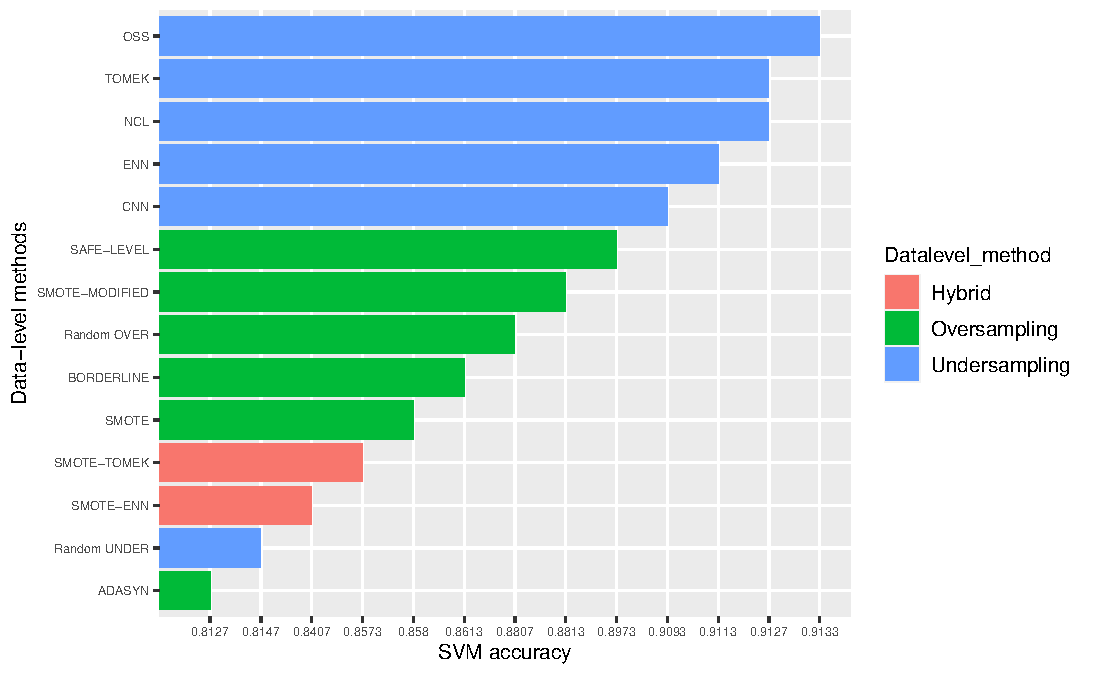
\includegraphics[width=1.1\textwidth]{Tesi_GabrieleCola/img/churn5.pdf}
\caption{Accuracy of data-level methods}
\end{center}



\section{Spam Detection}
Spam Dataset contains fifty-eight variables,which explain the features of email.  \\
The first 48 variables contain the frequency of the variable name in the e-mail.  \\
 Variables 49-54 indicate the frequency of the characters. \\
 Variables 55-57 contain the average, longest and total run-length of capital letters. \\
The variable 58 indicates the type of the mail and is either "nonspam" or "spam".\\

In this dataset, differently from Churn dataset, all cost-sensitive algorithms are applied. Thus, no data pre-processing is performed. A modified algorithm is used to predict if an email will go to the spam box or not. \\

\begin{center}
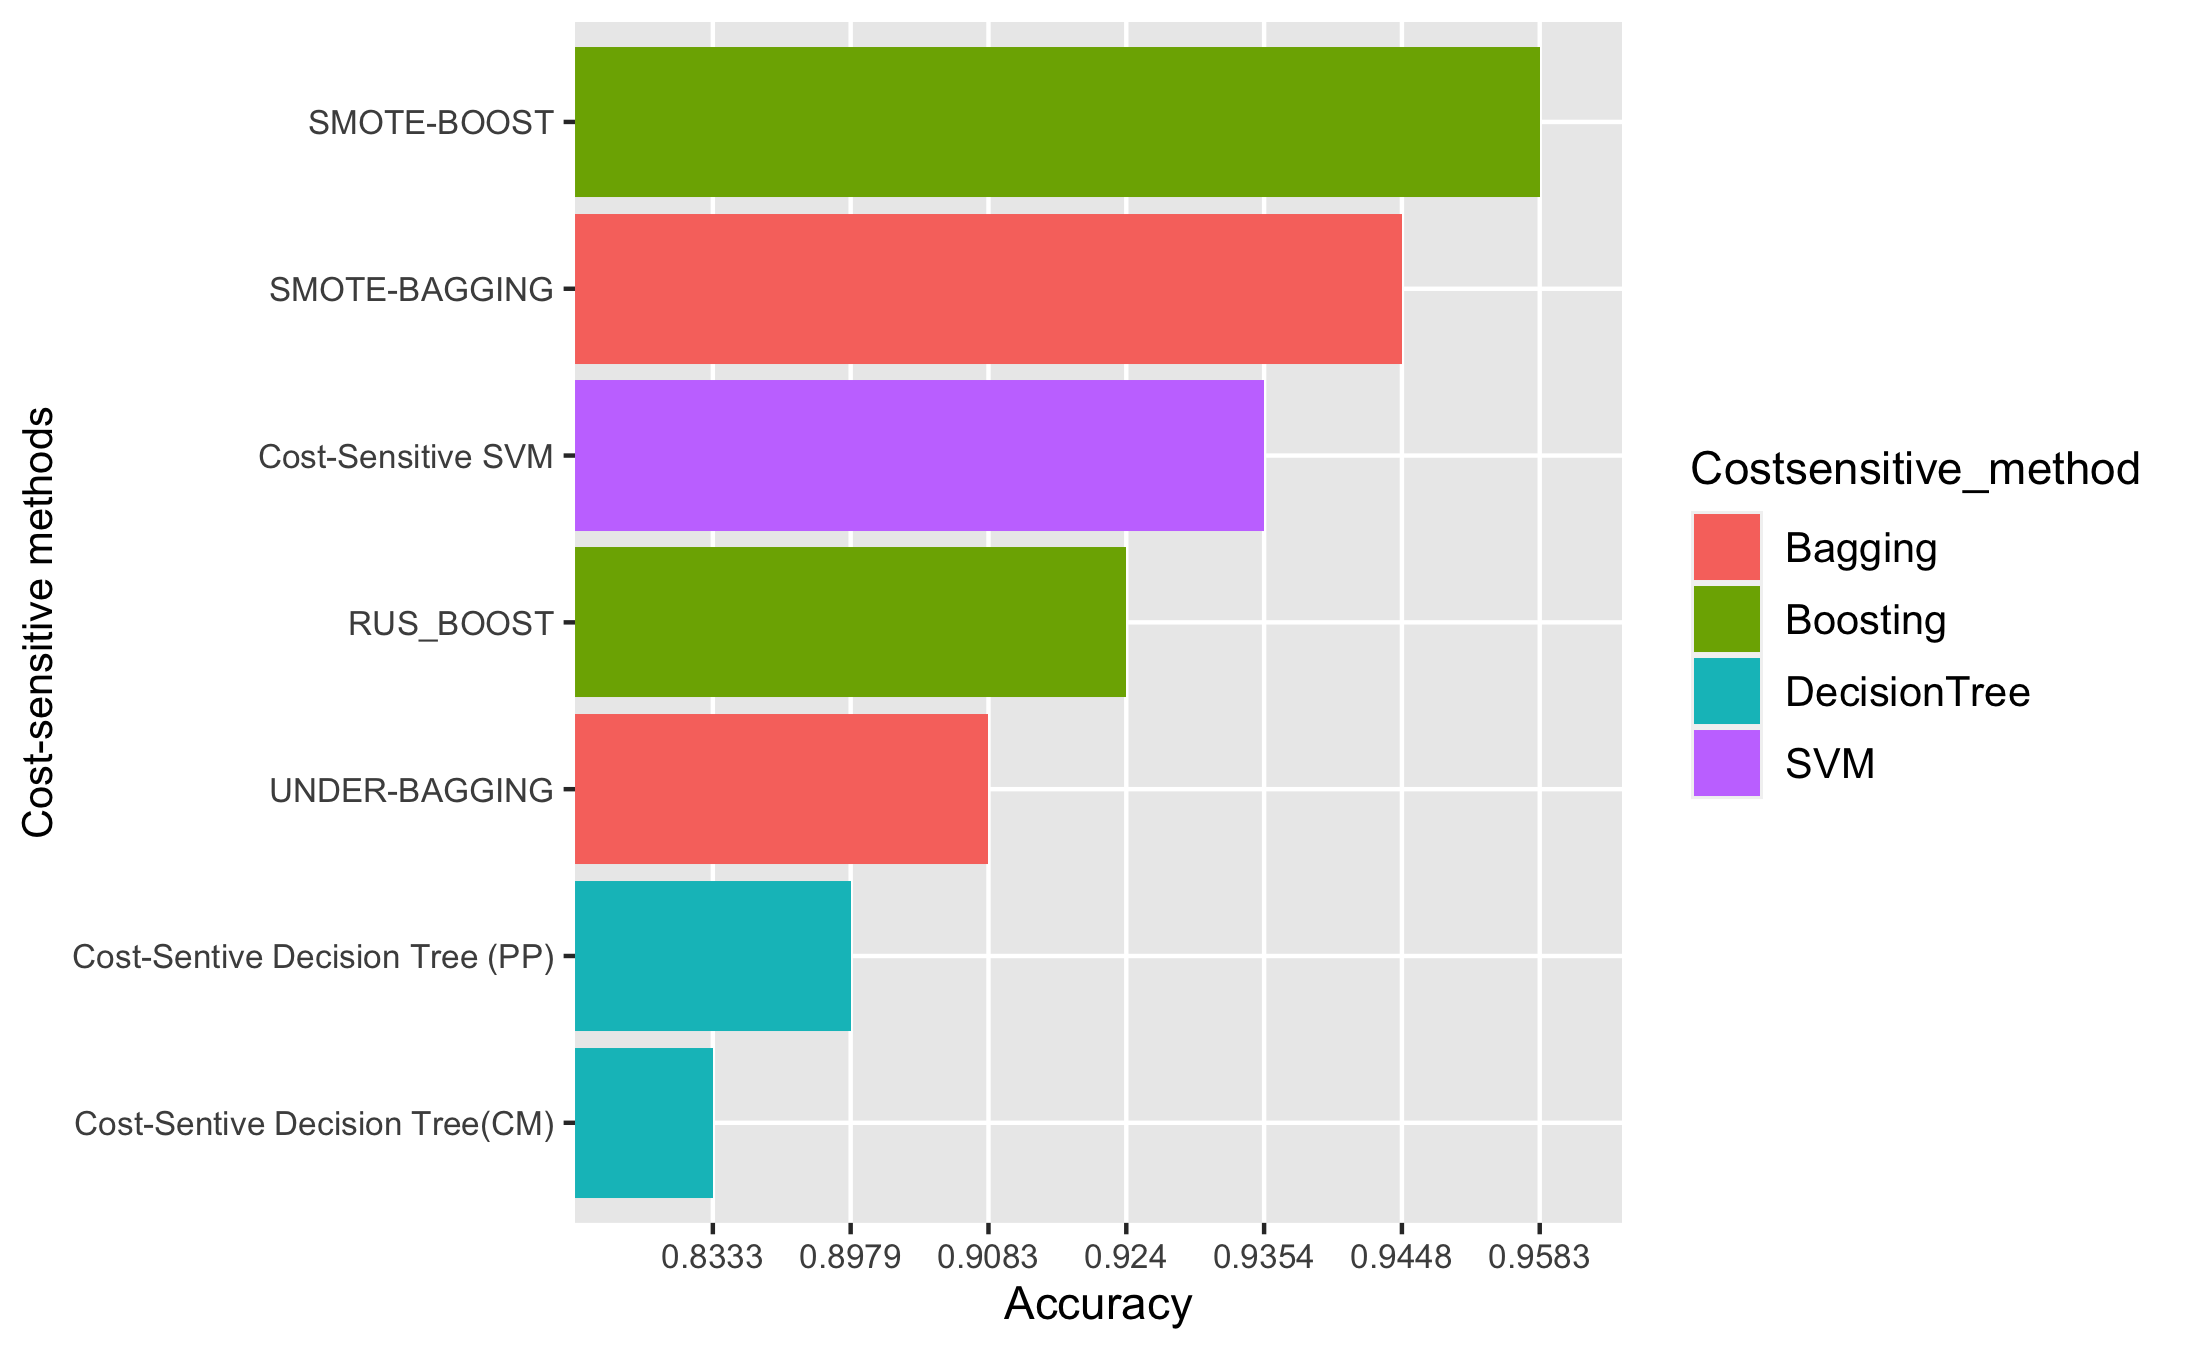
\includegraphics[width=1.1\textwidth]{Tesi_GabrieleCola/img/spam5.png}
\caption{Accuracy of cost-sensitive methods}
\end{center}



    
    



